% The two-route pipeline diagram (Figure 4.1), pre-rendered so that main.tex
% does not load TikZ. Regenerate with pdfLaTeX, then copy pipeline.pdf to figures/.
\documentclass[12pt,border=2pt]{standalone}
\usepackage[T1]{fontenc}
\usepackage{lmodern}
\usepackage{tikz}
\usetikzlibrary{positioning,arrows.meta,calc}
\begin{document}
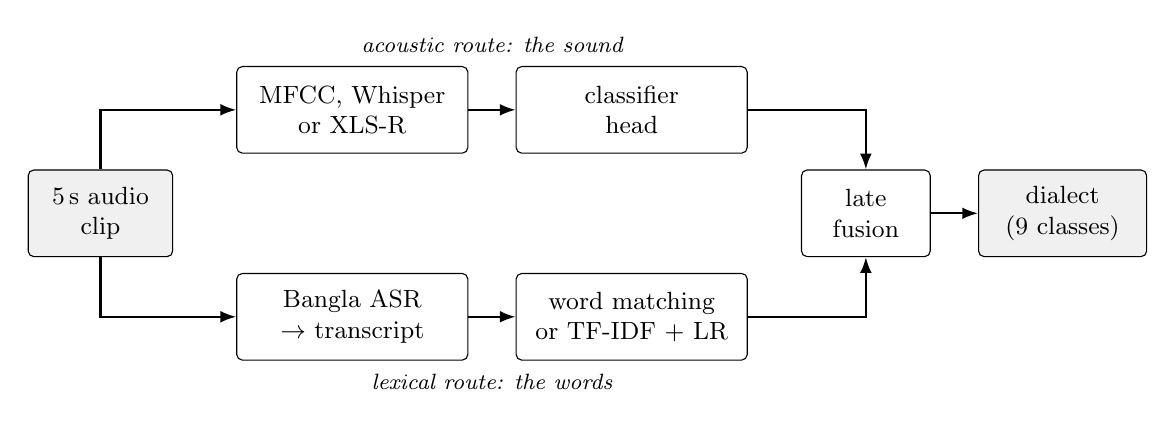
\begin{tikzpicture}[
    node distance=5mm and 6mm,
    box/.style={draw, rounded corners=2pt, align=center, font=\small,
                minimum height=11mm, text width=27mm, fill=white},
    data/.style={box, fill=black!6, text width=16mm},
    arr/.style={-{Latex[length=2mm]}, thick}]
  \node[data] (audio) {5\,s audio clip};
  \node[box, above right=2mm and 8mm of audio] (enc) {MFCC, Whisper\\or XLS-R};
  \node[box, right=of enc] (aclf) {classifier\\head};
  \node[box, below right=2mm and 8mm of audio] (asr) {Bangla ASR\\$\rightarrow$ transcript};
  \node[box, right=of asr] (lclf) {word matching\\or TF-IDF + LR};
  \node[box, text width=14mm] (fuse) at ($(aclf.east)!0.5!(lclf.east) + (15mm,0)$) {late\\fusion};
  \node[data, right=6mm of fuse, text width=19mm] (out) {dialect\\(9 classes)};
  \draw[arr] (audio.north) |- (enc.west);
  \draw[arr] (enc) -- (aclf);
  \draw[arr] (audio.south) |- (asr.west);
  \draw[arr] (asr) -- (lclf);
  \draw[arr] (aclf.east) -| (fuse.north);
  \draw[arr] (lclf.east) -| (fuse.south);
  \draw[arr] (fuse) -- (out);
  \node[font=\footnotesize\itshape, anchor=south, yshift=0.5mm] at ($(enc.north)!0.5!(aclf.north)$) {acoustic route: the sound};
  \node[font=\footnotesize\itshape, anchor=north, yshift=-0.5mm] at ($(asr.south)!0.5!(lclf.south)$) {lexical route: the words};
\end{tikzpicture}
\end{document}
